\documentclass{article}
\usepackage[utf8]{inputenc}
\usepackage{amsmath}
\usepackage{amsfonts}
\usepackage{amssymb}
\usepackage{graphicx}
\usepackage{geometry}
\usepackage{xcolor}
\usepackage{gensymb}
\usepackage{hyperref}
\usepackage{gensymb}
\usepackage{listings}

\newcommand{\inv}{^{-1}}   
\newcommand{\Z}{\mathbb Z}
\newcommand{\R}{\mathbb R}
\newcommand{\Q}{\mathbb Q}
\newcommand{\C}{\mathbb C}
\newcommand{\N}{\mathbb N}

\begin{document}

\medskip\noindent\textbf{1.} 

    \begin{center} 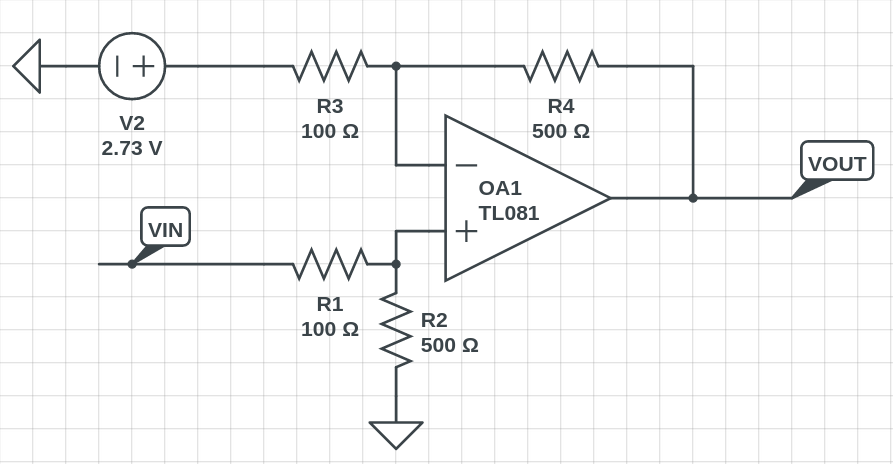
\includegraphics[scale=.7]{1.png} \end{center}

\medskip\noindent\textbf{2.} 

    The open circuit voltage is 6.666V.
    This is because the 1k resistors can be combined into a single 2k resistor, and the 4k resistor that goes to Vout will have no current at all, so we expect a 1/3 voltage drop across the combined 1k resistors.
    
    The short circuit current is $\frac1{800}$A.
    This is because the 4k resistors will receive an even split of the current coming through the 2k resistor, and V=IR tells us that the current through the 2k resistor is $\frac1{400}$A.

    Thus, the Thévenin equivalent circuit consists of a 6.666V voltage source and a 5333$\Omega$ resistor.

\newpage\noindent\textbf{3.}

    \begin{center} 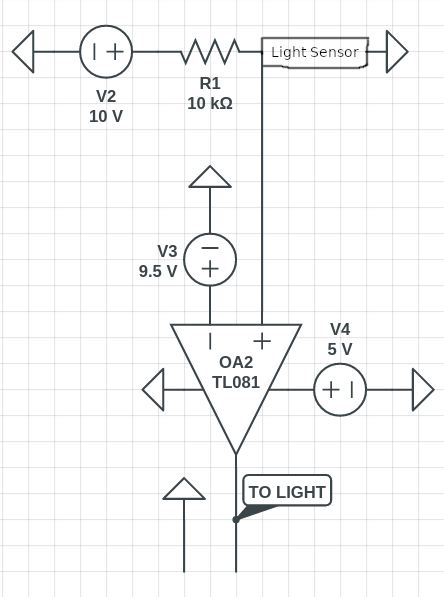
\includegraphics{2.png} \end{center}

    When it's dark, the light sensor will act as a 10k$\Omega$ resistor, so we'd expect to see 5V on the non-inverting input of the comparator.
    When it's bright, the light sensor will act as a >1M$\Omega$ resistor, so we'd expect to see upwards of 9.9V on the non-inverting input of the comparator.
    Still, I made my cutoff voltage for the comparator 9.5V; I don't want to waste electricity turning a light on when it's bright out.

\newpage\noindent\textbf{4.}

    As written, the code would print a value around $(V_1/3.3) \cdot 65535$, where $V_1$ is the voltage on A0. (Because the question says the voltage was applied on A1)
    But I think the answer you're looking for is that the code would print a value around $(1.25/3.3) \cdot 65535 \approx 24824$, and that the A0/A1 thing is just a typo.

\medskip\noindent\textbf{5.}

    The cut-off frequency for this low pass filter is $\frac{1}{2\pi\cdot11000000\cdot 20 \cdot 10^{-12}} \approx 723.43$Hz.
    Thus, the oscilloscope will be able to measure frequencies from 0Hz - 723Hz without too much loss.
    This seems like a pretty weak oscilloscope.

\medskip\noindent\textbf{6.}
\begin{verbatim}
import board
from analogio import AnalogIn
from digitalio import DigitalInOut, Direction
from time import sleep

a = AnalogIn(board.A1)
d = DigitalInOut(board.D4)
d.direction = Direction.INPUT

while True:
    if not d.value:
        print(a.value / 65535 * 3.3)
    sleep(.5)
\end{verbatim}

\newpage\noindent\textbf{7.}

    The golden rules tell us that the inputs to the op-amp will have the same voltage.
    Since the current through $R_1$ is equal to $I_L$, and the current through $R_2$ is equal to the current through the 5k resistor, we can solve for $V_{out}$ in terms of $I_L$, $R_1$ and $R_2$ to find that $$\frac{5000I_LR_1}{R_2} = V_o$$

    \begin{center} 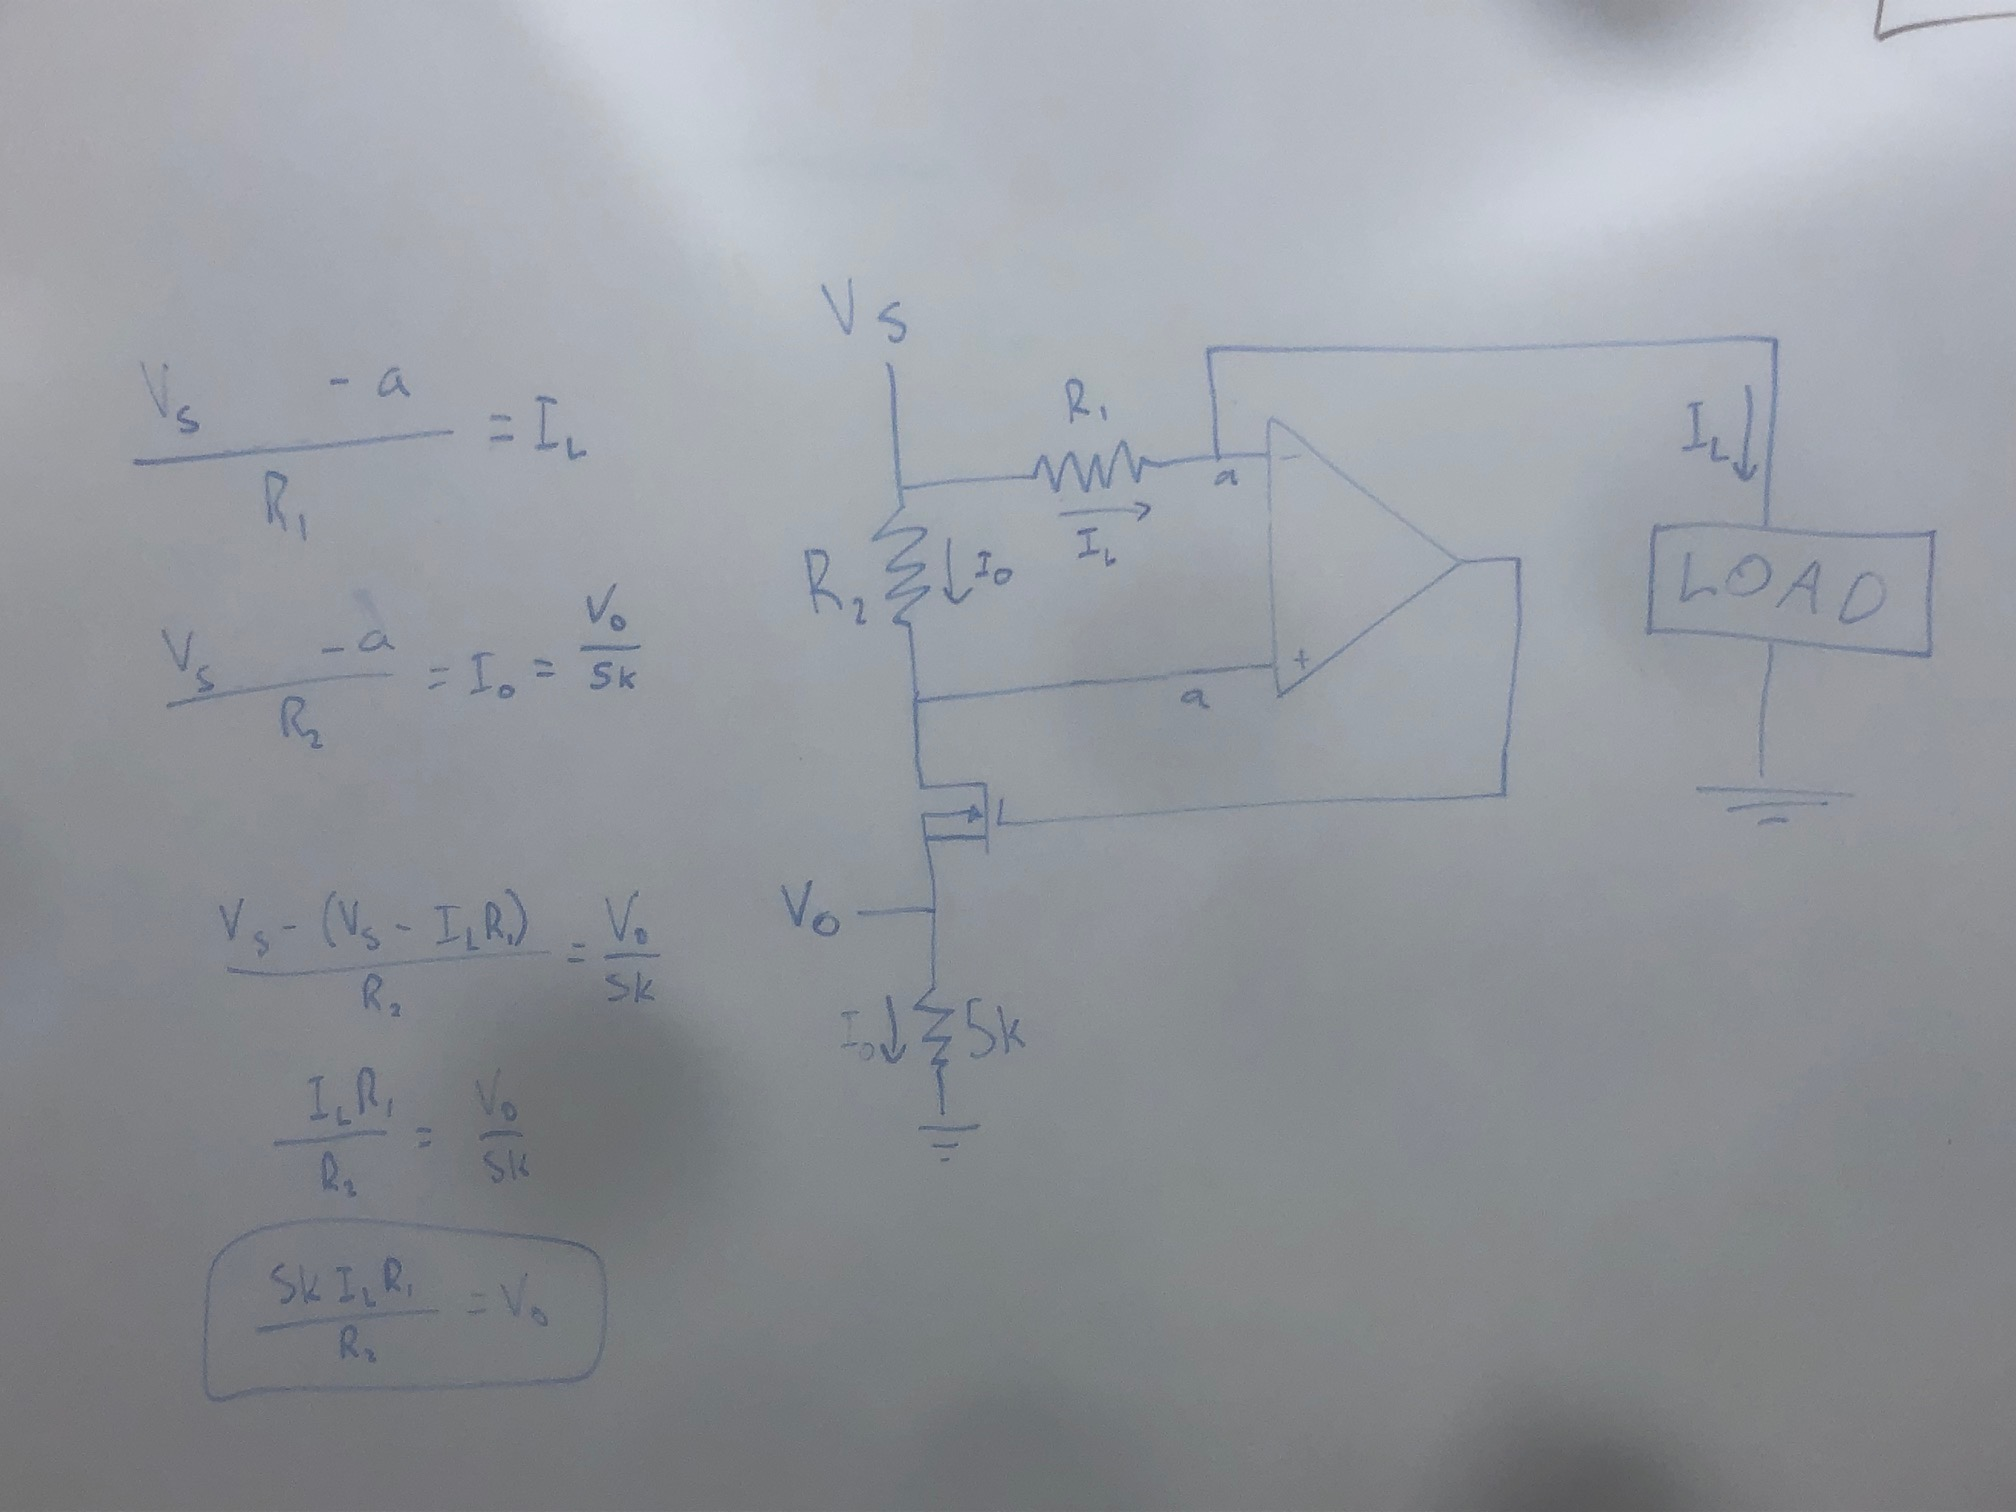
\includegraphics[scale=.2]{3.jpg} \end{center}

    This circuit works because the op-amp plays with the FET so that the op-amp's inputs have the same voltage.
    Because the voltage of the inverting input is determined by the resistance of the load (and thus $I_L$), and the two inputs must have the same voltage, the current through $R_2$ is also determined by $I_L$.
    Because the current through $R_2$ is equal to the current through the 5k resistor, the current through $R_2$ (and thus $I_L$) determines $V_o$.

\newpage\noindent\textbf{8.}

    \begin{center} 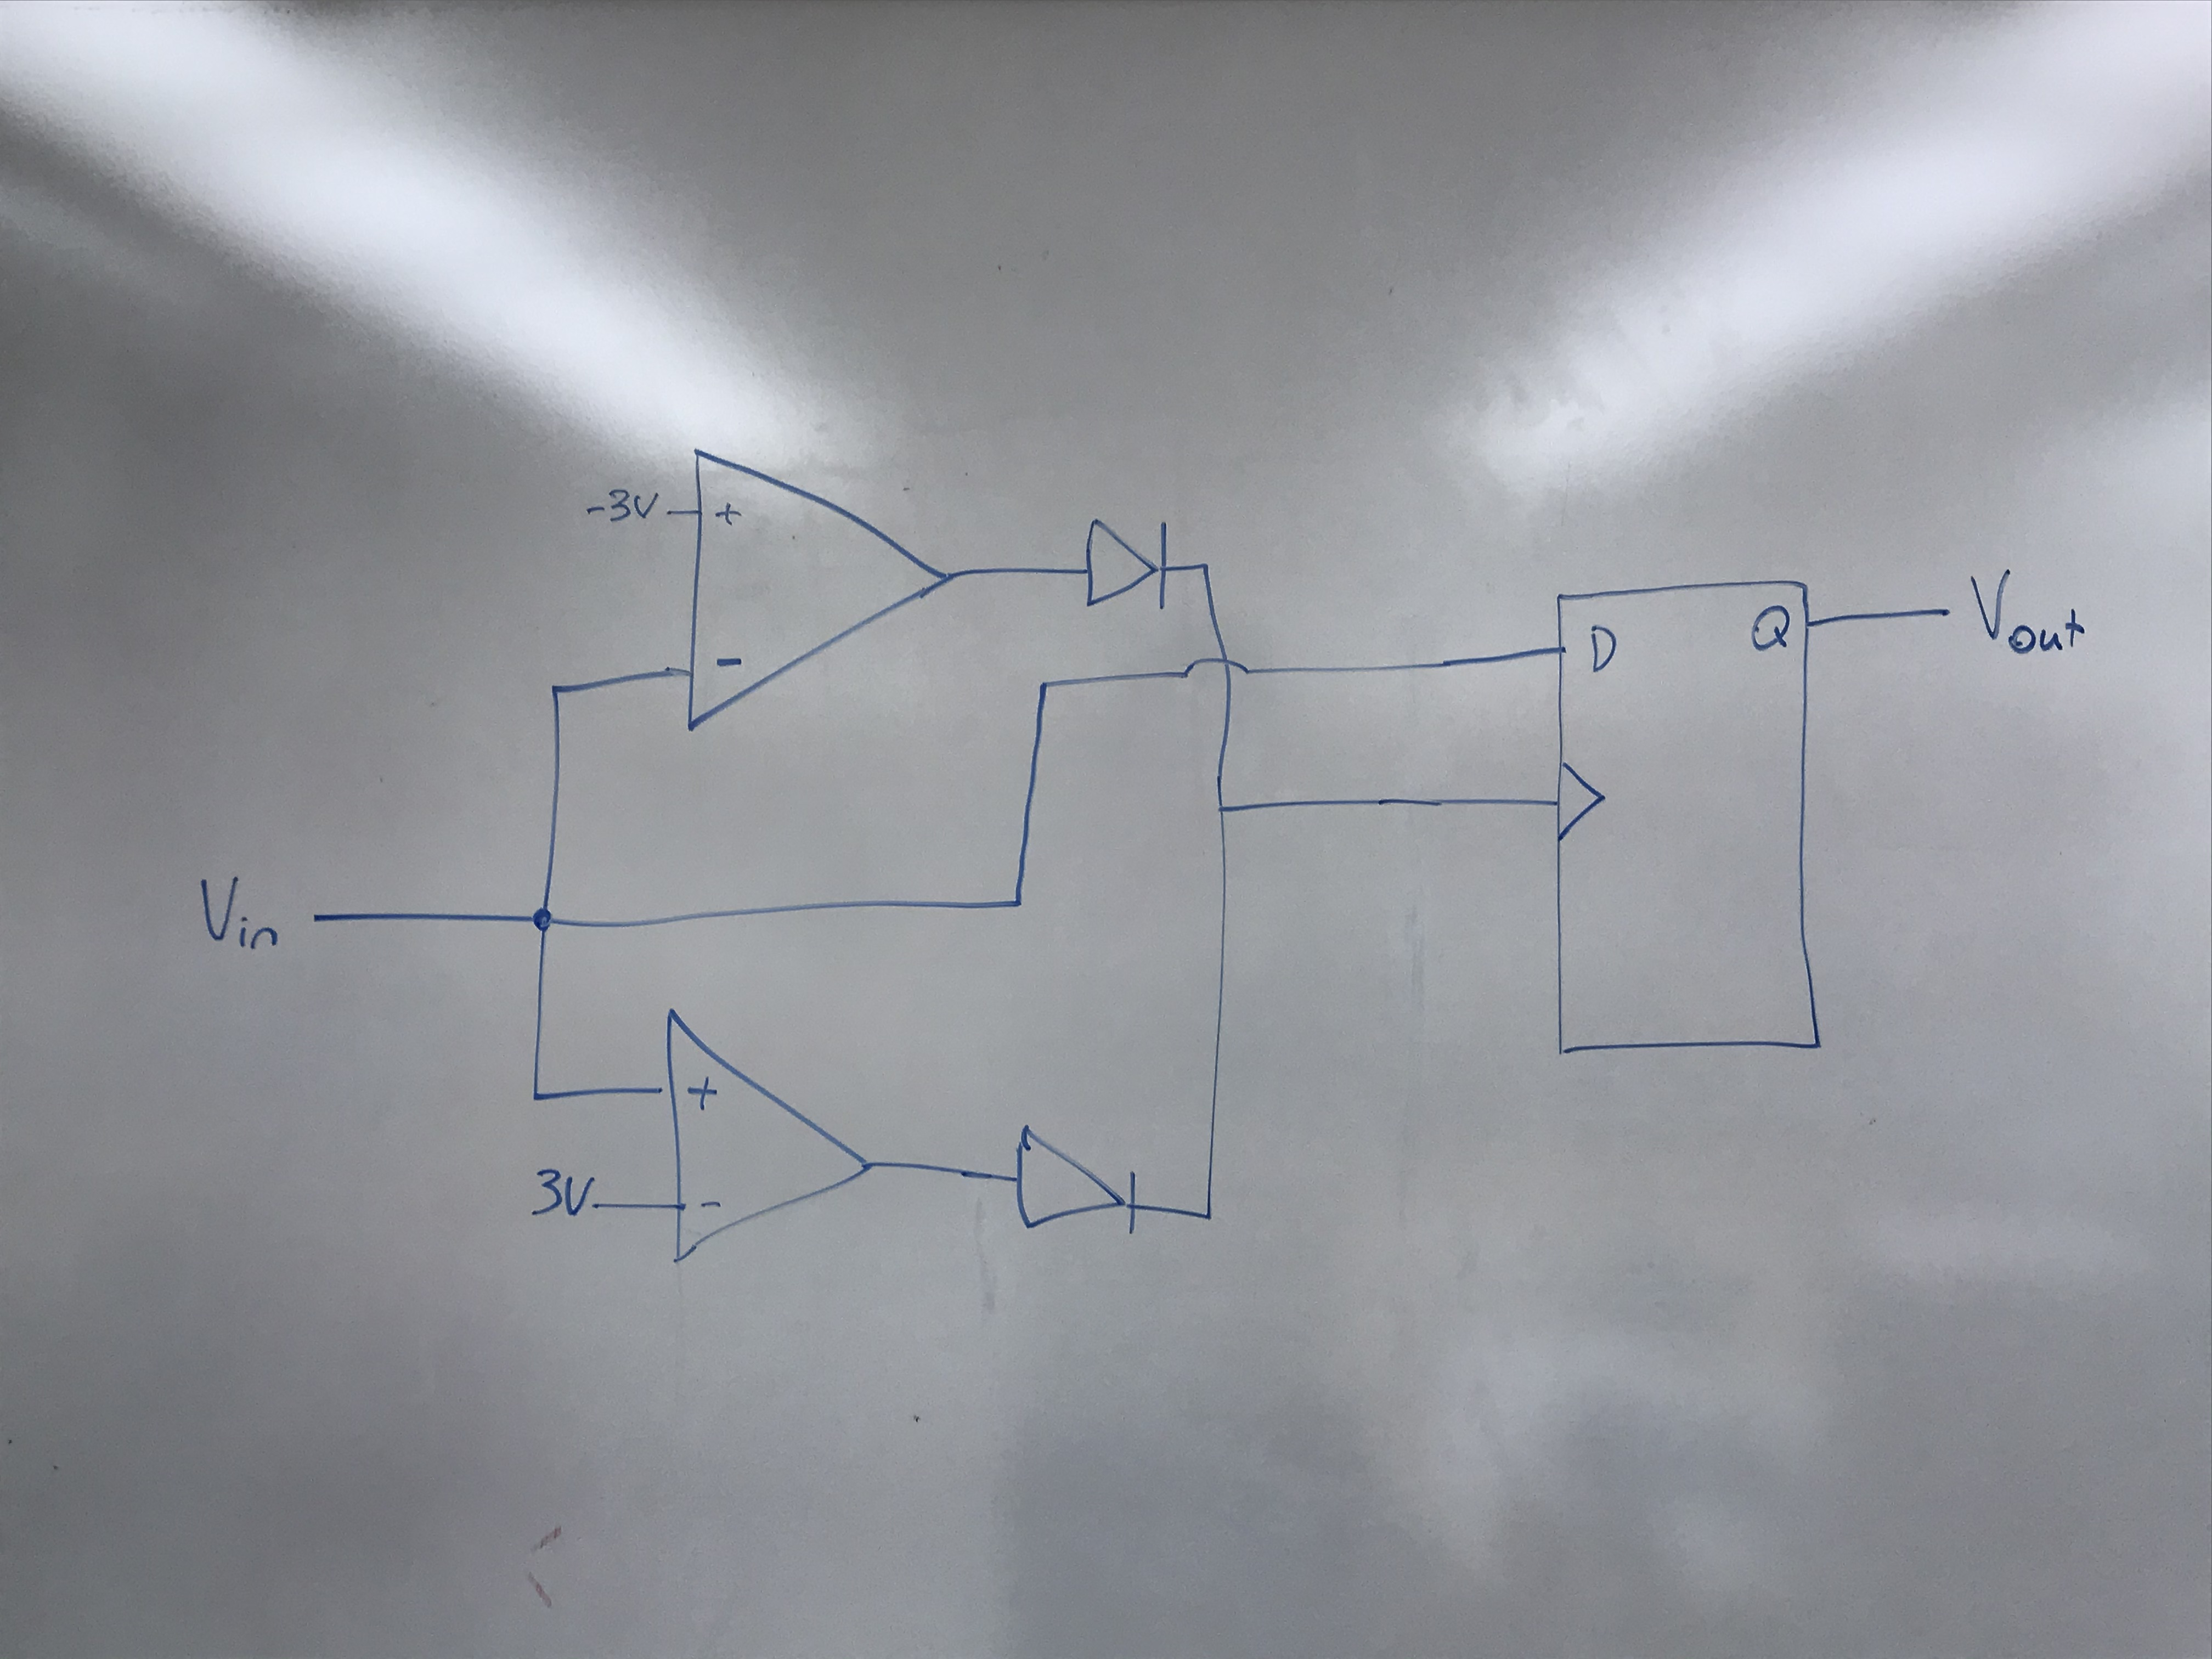
\includegraphics[scale=.12]{4.jpg} \end{center}

    This works because the clock input will be make a 0-1 transition when the voltage dips below -3V or rises above 3V.
    During those moments, the D-type flip-flop sets its output based on Vin.
    Thus, when Vin jumps above 3V, the clock triggers and the output is set high, and when Vin dips below -3V, the clock triggers again and the output is set low.

\end{document}
